\pgfplotsset{
    width=\textwidth*0.45,
    tick label style={font=\footnotesize},
    label style={font=\small},
    legend style={font=\tiny},
}

% Example of a figure that spans the whole page width and with subfigures. The same concept works for tables, too.
\begin{figure}[htb]
%\isPreprints{}{% This command is only used for ``preprints''.
%\begin{adjustwidth}{-\extralength}{0cm}
\centering
%} % If the paper is ``preprints'', please uncomment this parenthesis.
\subfloat[\centering]{
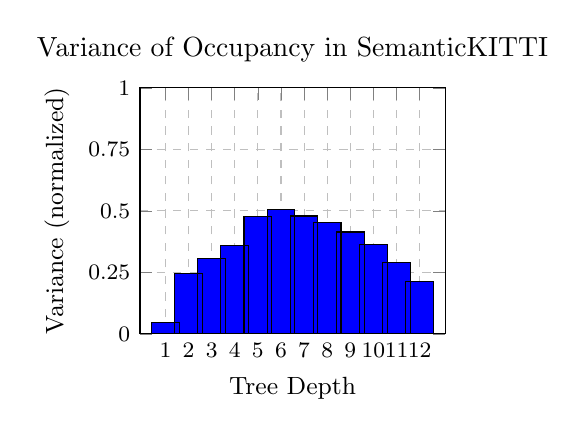
\begin{tikzpicture}
\begin{axis}[
    title={Variance of Occupancy in SemanticKITTI},
    xlabel={Tree Depth},
    ylabel={Variance (normalized)},
    symbolic x coords={1,2,3,4,5,6,7,8,9,10,11,12},
    xtick=data,
    %xmin=0, xmax=12,
    ymin=0, ymax=1.0,
    %xtick=data,
    ytick={0.0,0.25,0.5,0.75,1.0},
    xmajorgrids=true,
    ymajorgrids=true,
    grid style=dashed,
]

\addplot[
    ybar,
    fill=blue
]
coordinates {
    (1,  0.04595424)
    (2,  0.24564731)
    (3,  0.30522503)
    (4,  0.35757483)
    (5,  0.47618924)
    (6,  0.50649685)
    (7,  0.47918713)
    (8,  0.45111252)
    (9,  0.41432945)
    (10,  0.36336878)
    (11,  0.28927699)
    (12,  0.21268709)
};    
\end{axis}
\end{tikzpicture}
}
\hfill
\subfloat[\centering]{
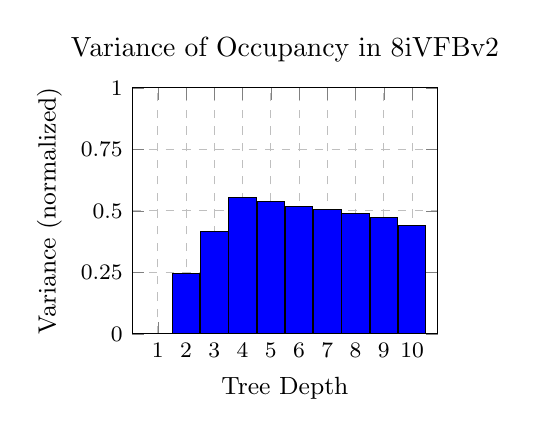
\begin{tikzpicture}
\begin{axis}[
    title={Variance of Occupancy in 8iVFBv2},
    xlabel={Tree Depth},
    ylabel={Variance (normalized)},
    symbolic x coords={1,2,3,4,5,6,7,8,9,10},
    xtick=data,
    ymin=0, ymax=1.0,
    %xtick=data,
    ytick={0.0,0.25,0.5,0.75,1.0},
    xmajorgrids=true,
    ymajorgrids=true,
    grid style=dashed,
]

\addplot[
    ybar,
    fill=blue
]
coordinates {
    (1, 0.0)
    (2, 0.24456905)
    (3, 0.41581164)
    (4, 0.55556464)
    (5, 0.53706259)
    (6, 0.5164308)
    (7, 0.50496453)
    (8, 0.49014243)
    (9, 0.47307183)
    (10, 0.43909567)
};    
\end{axis}
\end{tikzpicture}
}

%\isPreprints{}{% This command is only used for ``preprints''.
%\end{adjustwidth}
%} % If the paper is ``preprints'', please uncomment this parenthesis.
\caption{
Variance in occupancy distributions across octree levels.
(\textbf{a}) SemanticKITTI (sparse): entropy is low at shallow and deep levels, but peaks at mid-levels where structural variation is highest.
(\textbf{b}) 8iVFBv2 (dense): occupancy distributions maintain consistently high variance starting from level 4 due to dense and surface-complete geometry.}
\label{fig:variance_plot}
\end{figure} 

% KITTI VarMean: [0.04595424 0.24564731 0.30522503 0.35757483 0.47618924 0.50649685 0.47918713 0.45111252 0.41432945 0.36336878 0.28927699 0.21268709]
% MPEG: VarMean: [0.         0.24456905 0.41581164 0.55556464 0.53706259 0.5164308 0.50496453 0.49014243 0.47307183 0.43909567]